%!TEX root = ../Master.tex

\section{Hardware} % (fold)
\label{sec:hardware}

As mentioned in \autoref{sec:project_introduction} the focus of the project have been on the software implementations of theory learned throughout the course.
By using a Neato XV-11 vacuum cleaning robot in \autoref{fig:neato_xv11} which have a build-in lidar to sense its environment, and that implements functionality to move by some unit distance, most hardware concerns have been eliminated.\\
The lidar has a resolution of 360 measurements per revolution and can measure up to 5 meters.\\

The Neato robot has a serial interface accessable through a USB port on the back of the robot.
This means that there is no support for wirelessly communicating with the robot.

\begin{figure}[H]
\centering
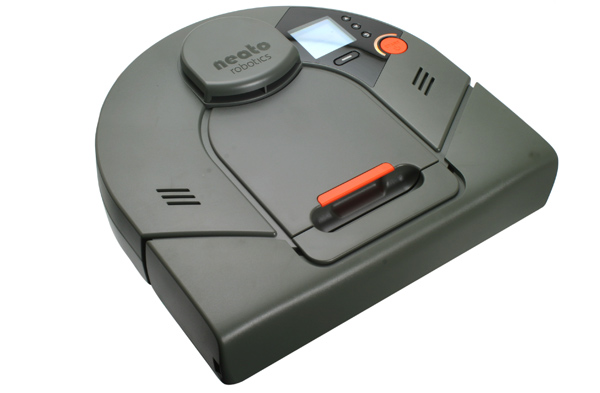
\includegraphics[scale=0.40]{images/neato_xv11}
\caption{Neato XV-11}
\label{fig:neato_xv11}
\end{figure}



% section hardware (end)
